\documentclass{article}
\usepackage{listings}
\usepackage[utf8x]{inputenc}
\usepackage[greek=nohyphenation,english=nohyphenation]{hyphsubst}
\usepackage[greek,english]{babel}
\usepackage{geometry}
%\usepackage{showframe} 
\newgeometry{vmargin={25mm}, hmargin={25mm,25mm}}
\usepackage{graphicx}
\graphicspath{ {./images/} }

\title{Numerical Analysis Second Project Report}
\author{Parmenion Charistos [3173]}
\date{January 2021}

\begin{document}
\maketitle

\section*{Introduction}
This report refers to the second mandatory project for the Numerical Analysis course given by the Aristotle university of Thessaloniki. Per exercise, adequate explanation and Matlab code snippets are provided. However, prerequisite knowledge on the subject is essential for its substantial comprehension.

\section{Part One}
The first task revolves around implementing three methods of locally approximating a function. These are the polynomial approach, the splines and the least squares method. To do so, 10 points of choice in the 2D space are selected to be used for the approximation. The sample function for testing is the $sin(x)$ in the interval $[-\pi,\pi]$. The selected points for our current example are given below; 
\[x = [-\pi,-3\pi/4,-\pi/2,-\pi/4,0,\pi/4,1,\pi/2,3\pi/4,\pi]\]
\[y = [0,-0.707,-1,-0.707,0,0.707,0.841,1,0.707,0];\]

\subsection{Polynomial Approach}
The polynomial approach involves the calculation via Lagrange interpolation. This is implemented via the following method;
\begin{lstlisting}[language=Matlab]

function res = Lagrange(x,y,targetX)
    n = length(x);
    L = ones(n,length(targetX));
    for i=1:1:n
        for j=1:1:n
            if i~=j
                L(i,:) = L(i,:).*(targetX - x(j))/(x(i) - x(j));
            end
        end
    end
    res = 0;
    for i=1:1:n
        res = res + y(i) * L(i,:);
    end
end
\end{lstlisting}
This method gets a set of \emph{x,y} sample coordinates and uses them to approximate the corresponding \emph{y} coordinates for the \emph{targetX} set of coordinates via the partial $L_i$ polynomials.
\pagebreak

\subsection{Splines}
No splines implementation could be made in time. An attempt to conclude results and a coding example on this method will be made in the future.

\subsection{Least Squares Method}
The least squares method (inaccurately referred to as minimal squares method in the code snippets), utilizes a sample of \emph{x,y} coordinates and approximates linearly the corresponding \emph{y} coordinates for the \emph{targetX} set of coordinates using polynomials of a given \emph{rank}. It computes the final matrix's row and column vectors and returns their product after inverting the former. This is achieved as follows;

\begin{lstlisting}[language=Matlab]
function resY = MinimumSquares(x,y,rank,targetX)
    %Initializing.
    rows = zeros(rank,rank);
    cols = zeros(rank,1);

    %Calculating row matrix.
    for i = 1:rank
        for j = 0:rank-1
            for k = 1:length(x)
               rows(i,j+1) = rows(i,j+1) + x(k)^(j+i-1);
            end
        end
    end

    %Calculating column vector
    for i = 1: rank
        for j = 1 : length(y)
            cols(i) = cols(i) + x(j)^(i-1) * y(j);
        end
    end

    %Returning approximations after calculating products.
    res = rows \ cols;
    resY = 0;
    for i=1:1:length(res)
        resY = resY + res(i)*targetX.^(i-1);
    end
end
\end{lstlisting}
\pagebreak
\subsection{Output}
The produced output for the given example via the previous methods is illustrated in this section.
\linebreak 
\begin{figure}[h]
\centering
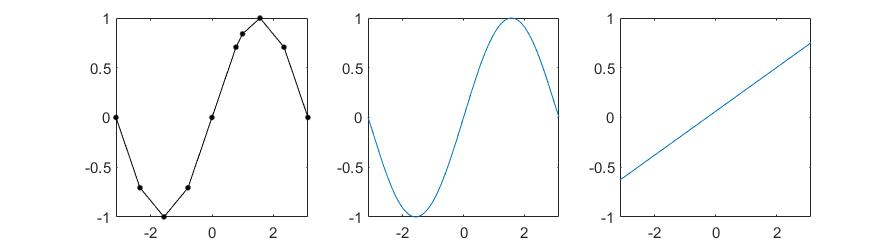
\includegraphics[scale=0.5]{images/sin_approx_figs.jpg}
\caption{From left to right, the first graph demonstrates the sample points used for the approximations, the second refers to the polynomial approach and last is the linear approximation via the least squares method.}
\end{figure}
\section{Part Two}
This part's assignments involved the implementation of the Simpson's method and the trapezoidal rule. These were, thus, utilized to calculate the definite integral of the $sin(x)$ function in the interval $[0,\pi/2]$.
\subsection{Simpson's Method}
This function takes as parameters a function handle \emph{f}, an interval's bounds \emph{a,b} and the number of parts \emph{n} the interval is divided in. Then, it follows the Simpson formula to approximate the target integral and finally printing it and the computation error for the current example.
\begin{lstlisting}[language=Matlab]
function [I,e] = Simpson(f,a,b,n)
    %Formula ingredients [disecting interval and calculating border values]
    h = (b-a)/n;
    q = f(a) + f(b);
   
    %Calculating the second multiplication operand for Simpson's Qn formula.
    for i=1:2:n-1
        q = q+4*f(a+i*h);
    end

    for i=2:2:n-2
        q = q+2*f(a+i*h);
    end
    
    %Calculating final approximated integral.
    I = h/3*q;

    %Calculating error for Simpson method.
    e = abs(1 - I);
end
\end{lstlisting}
\pagebreak
The result printed is;
\begin{lstlisting}[language=Matlab]
[Simpson Method]

I = 0.85817165
e = 0.14182835

I refers to the approximated definite integral of f.
e refers to the corresponding error of the approximation.
\end{lstlisting}
\subsection{Trapezoidal Rule}
This function implements the trapezoidal rule to approximate the integral of a function \emph{f} in the interval \emph{[a,b]} of \emph{n} partitions. Code-wise, it is demonstrated as follows;
\begin{lstlisting}[language=Matlab]
function [I,e] = Trapezoidal(f,a,b,n)
    %Disecting interval.
    h = (b - a)/n;
    x = a:h:b;
    I = 0;
    
    %Calculating integral according to trapezoidal rule.
    for i=1:1:n
        I = I + (x(i+1) - x(i))*(f(x(i+1)) + f(x(i)))/2;
    end
    
    e = abs(1 - I);
end
\end{lstlisting}
The occuring result is;
\begin{lstlisting}[language=Matlab]
[Trapezoid Method]

I = 0.99830011
e = 0.00169989

I refers to the approximated definite integral of f.
e refers to the corresponding error of the approximation.
\end{lstlisting}
\pagebreak
\section{Part Three}
In this section the tasks involved the prediction of the value of two stocks in a five day period, based on the past seven closes. The approximation was made via the least squares method to produce the following results.
\\*\\*In this example, data for two stocks (\foreignlanguage{greek}{ΔΕΗ, ΙΝΤΡΑΛΟΤ}) of the greek stock market were used. The dates used for approximation were from the week preceding the 13th November of the current year. These were included in the code, along with the actual values to be predicted, as shown;
\begin{lstlisting}[language=Matlab]
%Defining data for approximation base.
trainX = [7,8,9,10,11,12,13];
trainY_DEI = [5.07,5.06,5.49,5.5,5.595,5.595,5.55];
trainY_INLOT = [0.115,0.116,0.125,0.123,0.123,0.12,0.127];

%Defining actual values for comparison plots.
totalX = [7,8,9,10,11,12,13,14,15,16,17,18];
realY_DEI = [5.07,5.06,5.49,5.5,5.595,5.595,5.55,5.855,5.855,5.98,5.9,5.975];
realY_INLOT = [0.115,0.116,0.125,0.123,0.123,0.12,0.127,0.15,0.144,0.15,0.15,0.153];

targetX = [14,15,16,17,18];
\end{lstlisting}
The stocks' actual value changes for the entire period, starting from the beginning of the week of the sample data and ending in the fifth day to be predicted, is illustrated in the following figure;
\begin{figure}[h]
\centering
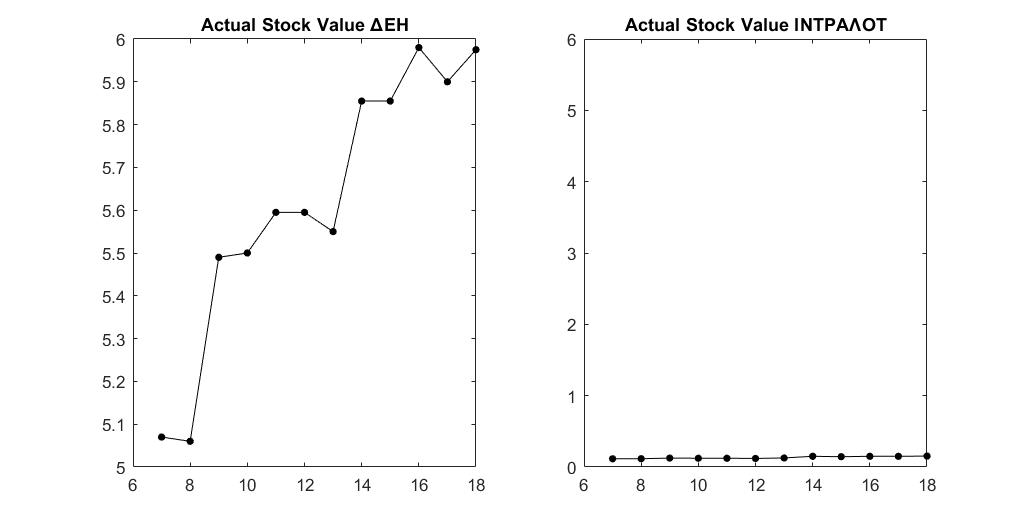
\includegraphics[scale=0.5]{images/actual_stock_values.jpg}
\end{figure}
\pagebreak 
\linebreak Using the least squares method described before, for polynomials of rank 2,3 and 4, the subsequent output is produced for the given data per each stock.
\begin{figure}[h]
\centering
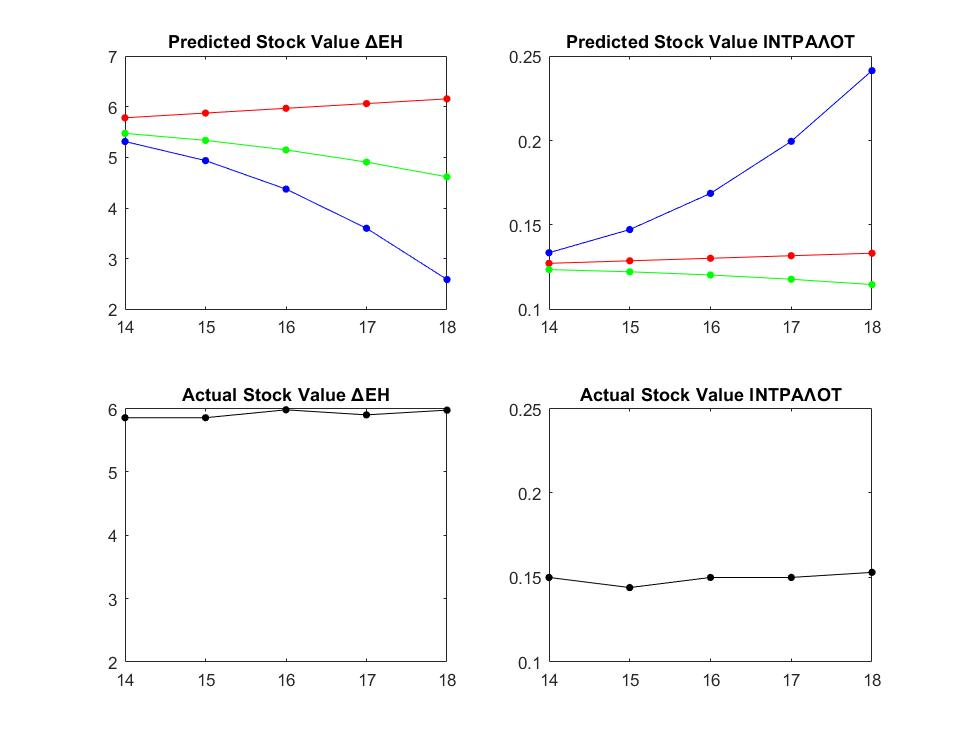
\includegraphics[scale=0.5]{images/stock_value_comparison.jpg}
\caption{The polynomials are color coded in a certain way. Red is rank-2, green is rank-3 and blue is rank-4.}
\end{figure}
\linebreak It is evident that the rank-2 polynomial was the most accurate in both cases, predicting very small value changes in the following days. In both the first and second cases, the rank-3 polynomial came out slightly pessimistic, predicting a small but steady drop in the stocks' values. However the rank-4 predicted vast drops in the case of the first stock and tremendous increase in value for the second one. It can be observed how the higher ranked polynomials gravitate more around the
\end{document}
